\section{lg\-Chord Class Reference}
\label{classlgChord}\index{lgChord@{lgChord}}
a chord based on {\bf lg\-Note}, containing a list of {\bf lg\-Voice}  


{\tt \#include $<$lgchord.h$>$}

Inheritance diagram for lg\-Chord::\begin{figure}[H]
\begin{center}
\leavevmode
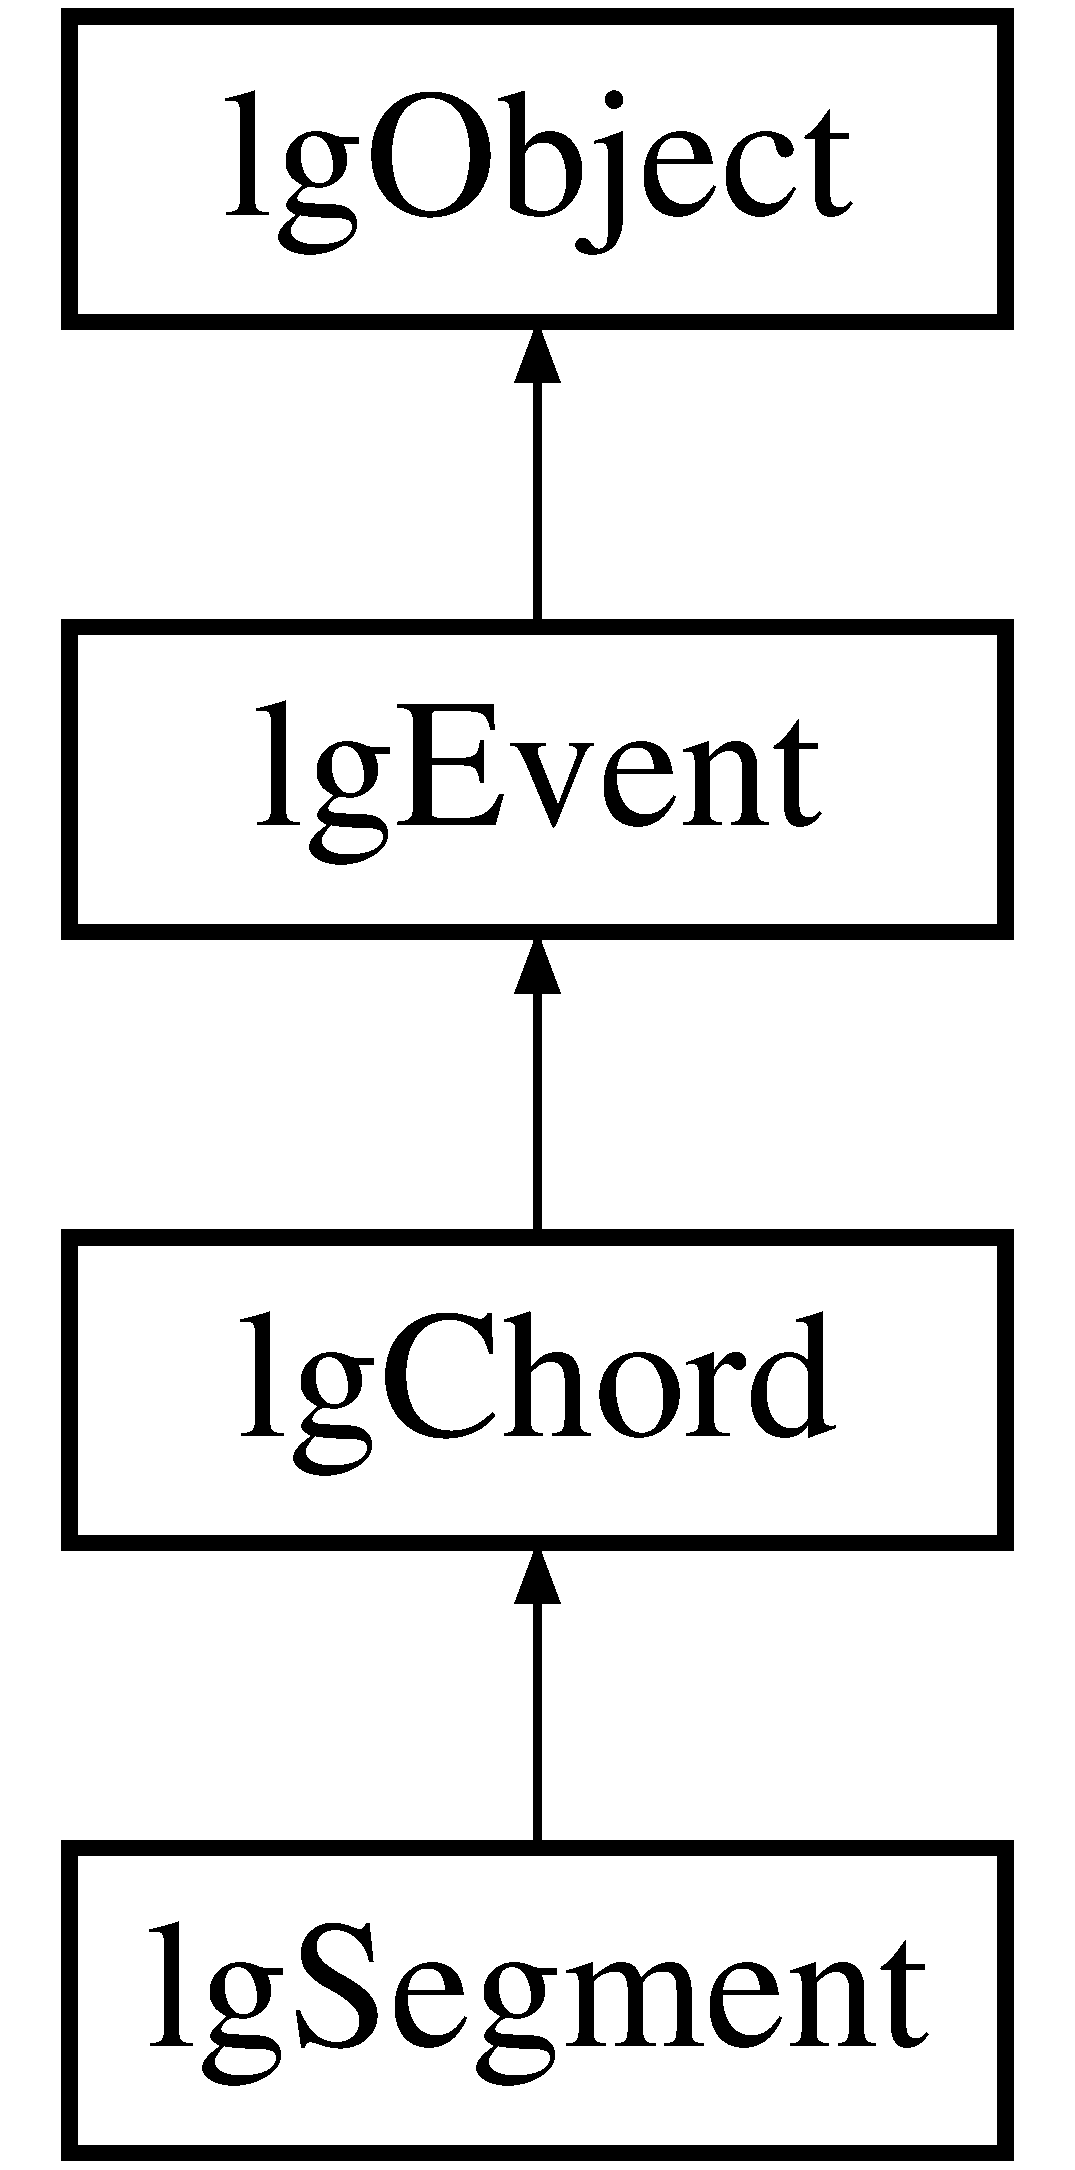
\includegraphics[height=4cm]{classlgChord}
\end{center}
\end{figure}
\subsection*{Public Member Functions}
\begin{CompactItemize}
\item 
void {\bf replace\-Range\-Ptr} ({\bf lg\-Event} $\ast$old, {\bf lg\-Event} $\ast$new\-Ev)
\begin{CompactList}\small\item\em replace in all tags with prev\-Ev\-I==old\-Ev, prev\-Ev by new\-Ev \item\end{CompactList}\item 
{\bf lg\-Chord} (long int pos\-Num, long int pos\-Denom)
\item 
virtual {\bf $\sim$lg\-Chord} (void)
\item 
virtual void {\bf append\-Event} ({\bf lg\-Event} $\ast$ev)
\begin{CompactList}\small\item\em append an event to voices\-Tail \item\end{CompactList}\item 
void {\bf append\-Voice} ({\bf lg\-Voice} $\ast$voice)
\item 
{\bf lg\-Voice} $\ast$ {\bf first\-Voice} (void)
\item 
virtual string {\bf to\-String} ({\bf lg\-Voice} $\ast$call\-Seq)
\begin{CompactList}\small\item\em reset the close\-Range stack for events/tags of all voices \item\end{CompactList}\item 
virtual void {\bf write} (FILE $\ast$out, {\bf lg\-Voice} $\ast$call\-Seq)
\begin{CompactList}\small\item\em write own data AND all tags starting in call\-Seq in (this-$>$pos...next-$>$pos] \item\end{CompactList}\item 
{\bf lg\-Tag} $\ast$ {\bf find\-Tag} (char $\ast$tag\-Name)
\begin{CompactList}\small\item\em search for a tag in all voices \item\end{CompactList}\item 
virtual {\bf lg\-Tag} $\ast$ {\bf find\-Tag} (long int id)
\begin{CompactList}\small\item\em search for a tag in all voices \item\end{CompactList}\item 
int {\bf split\-Tag\-Ranges} (void)
\begin{CompactList}\small\item\em split all explicit tag ranges (using \char`\"{}(....\char`\"{}) ) into $\backslash$...Begin and $\backslash$...End and return number of changed ranges \item\end{CompactList}\end{CompactItemize}
\subsection*{Protected Attributes}
\begin{CompactItemize}
\item 
{\bf lg\-Voice} $\ast$ {\bf voices\-I}
\item 
{\bf lg\-Voice} $\ast$ {\bf voices\-Tail}
\end{CompactItemize}


\subsection{Detailed Description}
a chord based on {\bf lg\-Note}, containing a list of {\bf lg\-Voice} 



\subsection{Constructor \& Destructor Documentation}
\index{lgChord@{lg\-Chord}!lgChord@{lgChord}}
\index{lgChord@{lgChord}!lgChord@{lg\-Chord}}
\subsubsection{\setlength{\rightskip}{0pt plus 5cm}lg\-Chord::lg\-Chord (long int {\em pos\-Num}, long int {\em pos\-Denom})}\label{classlgChord_a1}


\index{lgChord@{lg\-Chord}!~lgChord@{$\sim$lgChord}}
\index{~lgChord@{$\sim$lgChord}!lgChord@{lg\-Chord}}
\subsubsection{\setlength{\rightskip}{0pt plus 5cm}lg\-Chord::$\sim${\bf lg\-Chord} (void)\hspace{0.3cm}{\tt  [virtual]}}\label{classlgChord_a2}




\subsection{Member Function Documentation}
\index{lgChord@{lg\-Chord}!appendEvent@{appendEvent}}
\index{appendEvent@{appendEvent}!lgChord@{lg\-Chord}}
\subsubsection{\setlength{\rightskip}{0pt plus 5cm}void lg\-Chord::append\-Event ({\bf lg\-Event} $\ast$ {\em ev})\hspace{0.3cm}{\tt  [virtual]}}\label{classlgChord_a3}


append an event to voices\-Tail 



Reimplemented in {\bf lg\-Segment} {\rm (p.\,\pageref{classlgSegment_a6})}.\index{lgChord@{lg\-Chord}!appendVoice@{appendVoice}}
\index{appendVoice@{appendVoice}!lgChord@{lg\-Chord}}
\subsubsection{\setlength{\rightskip}{0pt plus 5cm}void lg\-Chord::append\-Voice ({\bf lg\-Voice} $\ast$ {\em v})}\label{classlgChord_a4}


append voice to chord, voices\-Tail must be up to date! \begin{Desc}
\item[Parameters: ]\par
\begin{description}
\item[{\em 
v}]sequence or voice \end{description}
\end{Desc}
\index{lgChord@{lg\-Chord}!findTag@{findTag}}
\index{findTag@{findTag}!lgChord@{lg\-Chord}}
\subsubsection{\setlength{\rightskip}{0pt plus 5cm}{\bf lg\-Tag} $\ast$ lg\-Chord::find\-Tag (long int {\em id})\hspace{0.3cm}{\tt  [virtual]}}\label{classlgChord_a9}


search for a tag in all voices 

\index{lgChord@{lg\-Chord}!findTag@{findTag}}
\index{findTag@{findTag}!lgChord@{lg\-Chord}}
\subsubsection{\setlength{\rightskip}{0pt plus 5cm}{\bf lg\-Tag} $\ast$ lg\-Chord::find\-Tag (char $\ast$ {\em tag\-Name})}\label{classlgChord_a8}


search for a tag in all voices 

\index{lgChord@{lg\-Chord}!firstVoice@{firstVoice}}
\index{firstVoice@{firstVoice}!lgChord@{lg\-Chord}}
\subsubsection{\setlength{\rightskip}{0pt plus 5cm}{\bf lg\-Voice}$\ast$ lg\-Chord::first\-Voice (void)\hspace{0.3cm}{\tt  [inline]}}\label{classlgChord_a5}


\index{lgChord@{lg\-Chord}!replaceRangePtr@{replaceRangePtr}}
\index{replaceRangePtr@{replaceRangePtr}!lgChord@{lg\-Chord}}
\subsubsection{\setlength{\rightskip}{0pt plus 5cm}void lg\-Chord::replace\-Range\-Ptr ({\bf lg\-Event} $\ast$ {\em old}, {\bf lg\-Event} $\ast$ {\em new\-Ev})}\label{classlgChord_a0}


replace in all tags with prev\-Ev\-I==old\-Ev, prev\-Ev by new\-Ev 

\index{lgChord@{lg\-Chord}!splitTagRanges@{splitTagRanges}}
\index{splitTagRanges@{splitTagRanges}!lgChord@{lg\-Chord}}
\subsubsection{\setlength{\rightskip}{0pt plus 5cm}int lg\-Chord::split\-Tag\-Ranges (void)}\label{classlgChord_a10}


split all explicit tag ranges (using \char`\"{}(....\char`\"{}) ) into $\backslash$...Begin and $\backslash$...End and return number of changed ranges 

\index{lgChord@{lg\-Chord}!toString@{toString}}
\index{toString@{toString}!lgChord@{lg\-Chord}}
\subsubsection{\setlength{\rightskip}{0pt plus 5cm}string lg\-Chord::to\-String ({\bf lg\-Voice} $\ast$ {\em call\-Seq})\hspace{0.3cm}{\tt  [virtual]}}\label{classlgChord_a6}


reset the close\-Range stack for events/tags of all voices 

write all tags between this and next call\-Seq might be NULL for Segements 

Reimplemented from {\bf lg\-Event} {\rm (p.\,\pageref{classlgEvent_a1})}.

Reimplemented in {\bf lg\-Segment} {\rm (p.\,\pageref{classlgSegment_a21})}.\index{lgChord@{lg\-Chord}!write@{write}}
\index{write@{write}!lgChord@{lg\-Chord}}
\subsubsection{\setlength{\rightskip}{0pt plus 5cm}void lg\-Chord::write (FILE $\ast$ {\em out}, {\bf lg\-Voice} $\ast$ {\em call\-Seq})\hspace{0.3cm}{\tt  [virtual]}}\label{classlgChord_a7}


write own data AND all tags starting in call\-Seq in (this-$>$pos...next-$>$pos] 



Reimplemented from {\bf lg\-Event} {\rm (p.\,\pageref{classlgEvent_a8})}.

Reimplemented in {\bf lg\-Segment} {\rm (p.\,\pageref{classlgSegment_a22})}.

\subsection{Member Data Documentation}
\index{lgChord@{lg\-Chord}!voicesI@{voicesI}}
\index{voicesI@{voicesI}!lgChord@{lg\-Chord}}
\subsubsection{\setlength{\rightskip}{0pt plus 5cm}{\bf lg\-Voice}$\ast$ {\bf lg\-Chord::voices\-I}\hspace{0.3cm}{\tt  [protected]}}\label{classlgChord_p0}


\index{lgChord@{lg\-Chord}!voicesTail@{voicesTail}}
\index{voicesTail@{voicesTail}!lgChord@{lg\-Chord}}
\subsubsection{\setlength{\rightskip}{0pt plus 5cm}{\bf lg\-Voice} $\ast$ {\bf lg\-Chord::voices\-Tail}\hspace{0.3cm}{\tt  [protected]}}\label{classlgChord_p1}




The documentation for this class was generated from the following files:\begin{CompactItemize}
\item 
{\bf lgchord.h}\item 
{\bf lgchord.cpp}\end{CompactItemize}
